%%% LaTeX Template: Article/Thesis/etc. with colored headings and special fonts
%%%
%%% Source: http://www.howtotex.com/
%%% Feel free to distribute this template, but please keep to referal to http://www.howtotex.com/ here.
%%% February 2011
%%%
%%% Modified January 2016 by CDM

%%%  Preamble
\documentclass[11pt,letterpaper]{article}
\usepackage[margin=1.0in]{geometry}
\usepackage[T1]{fontenc}
\usepackage[bitstream-charter]{mathdesign}
\usepackage[latin1]{inputenc}					
\usepackage{amsmath}						
\usepackage{xcolor}
\usepackage{cite}
\usepackage{hyphenat}
\usepackage{graphicx}
\usepackage{float}
\usepackage{subfigure}
\usepackage{sectsty}
\usepackage[compact]{titlesec} 
\usepackage[tablegrid]{vhistory}
\usepackage{pbox}
\usepackage{wrapfig}
\usepackage[export]{adjustbox}
\allsectionsfont{\color{accentcolor}\scshape\selectfont}

%%% Definitions
\definecolor{accentcolor}{rgb}{0.0,0.0,0.5} 
\newcommand{\teamname}{Resonance}
\newcommand{\productname}{Ltunes}
\newcommand{\coursename}{CSE 4317: Senior Design II}
\newcommand{\semester}{Fall 2019}
\newcommand{\docname}{Detailed Design Specification}
\newcommand{\department}{Department of Computer Science \& Engineering}
\newcommand{\university}{The University of Texas at Arlington}
\newcommand{\authors}{Amir Dhungana \\ Anish Yonjan \\ Roberto Torres \\ Raul Jimenez \\ Rabinson Shrestha \\ Nikhil Purohit}

%%% Headers and footers
\usepackage{fancyhdr}
	\pagestyle{fancy}						% Enabling the custom headers/footers
\usepackage{lastpage}	
	% Header (empty)
	\lhead{}
	\chead{}
	\rhead{}
	% Footer
	\lfoot{\footnotesize \teamname \ - \semester}
	\cfoot{}
	\rfoot{\footnotesize page \thepage\ of \pageref{LastPage}}	% "Page 1 of 2"
	\renewcommand{\headrulewidth}{0.0pt}
	\renewcommand{\footrulewidth}{0.4pt}

%%% Change the abstract environment
\usepackage[runin]{abstract}			% runin option for a run-in title
%\setlength\absleftindent{30pt}			% left margin
%\setlength\absrightindent{30pt}		% right margin
\abslabeldelim{\quad}	
\setlength{\abstitleskip}{-10pt}
\renewcommand{\abstractname}{}
\renewcommand{\abstracttextfont}{\color{accentcolor} \small \slshape}	% slanted text

%%% Start of the document
\begin{document}

%%% Cover sheet
{\centering \huge \color{accentcolor} \sc \textbf{\department \\ \university} \par}
\vspace{1 in}
{\centering \huge \color{accentcolor} \sc \textbf{\docname \\ \coursename \\ \semester} \par}
\vspace{0.5 in}
\begin{figure}[h!]
	\centering
   	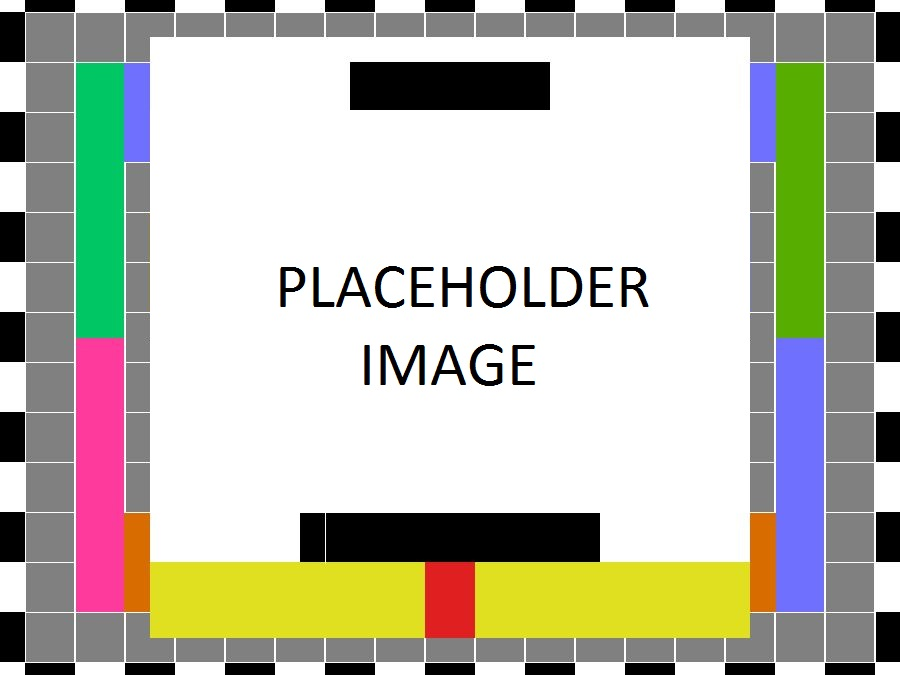
\includegraphics[width=0.60\textwidth]{images/test_image}
\end{figure}
\vspace{0.5 in}
{\centering \huge \color{accentcolor} \sc \textbf{\teamname \\ \productname} \par}
\vspace{0.5 in}
{\centering \large \sc \textbf{\authors} \par}
\newpage


%\vspace{1 in}
%\centerline{January 13th, 2012}
%\newpage

%%% Revision History
\begin{versionhistory}
  	\vhEntry{0.1}{02.14.2020}{AD}{document creation}
  	\vhEntry{0.2}{02.20.2020}{AD}{complete draft}
  	\vhEntry{0.3}{02.21.2020}{AD}{release candidate 1}
  	\vhEntry{1.0}{02.21.2020}{AD}{official release}
  	\vhEntry{1.1}{05.11.2020}{AD}{revision and update}
  	
  
\end{versionhistory}
\newpage

%%% Table of contents
\setcounter{tocdepth}{2}
\tableofcontents
\newpage

%%% List of figures and tables (optional)
\listoffigures
\listoftables
\newpage

%%% Document sections
\section{Introduction}
Your introduction should describe your product concept in sufficient detail that the architectural design will be easy to follow. The introduction may include information used in the first sections of your SRS for this purpose. At a minimum, ensure that the product concept, scope and key requirements are described.
\section{System Overview}
This section should reintroduce the full data flow diagram from the architectural specification, and discuss at a high level the purpose of each layer. You do not need to include a subsection for each layer, a 1 - 2 paragraph recap is sufficient.

\begin{figure}[h!]
	\centering
 	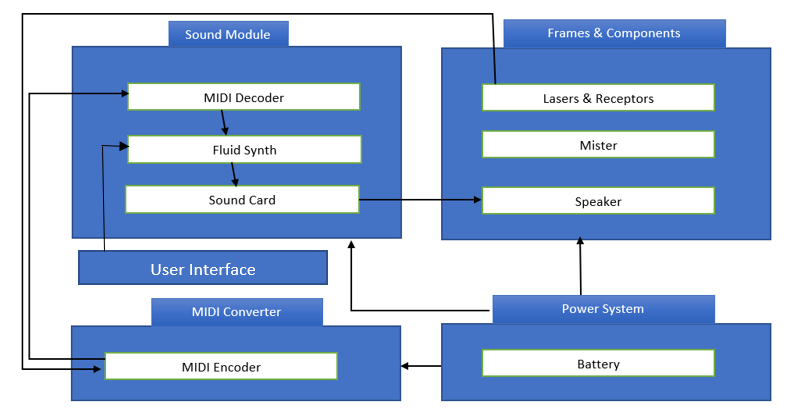
\includegraphics[width=0.90\textwidth]{images/data_flow}
 \caption{System architecture}
\end{figure}

\newpage
%\section{Subsystem Definitions \& Data Flow}
%This section breaks down your layer abstraction to another level of detail. Here you grapically represent the logical subsytems that compose each layer and show the interactions/interfaces between those subsystems. A subsystem can be thought of as a programming unit that implements one of the major functions of the layer. It, therefore, has data elements that serve as source/sinks for other subsystems. The logical data elements that flow between subsystems need to be explicitly defined at this point, beginning with a data flow-like diagram based on the block diagram.

\begin{figure}[h!]
	\centering
 	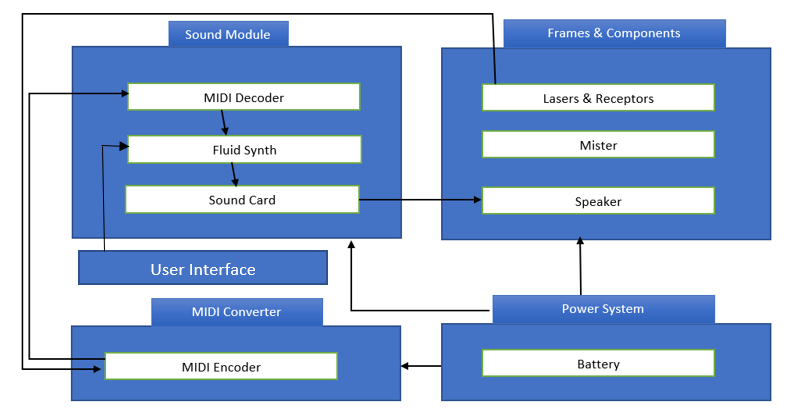
\includegraphics[width=\textwidth]{images/data_flow}
 \caption{A simple data flow diagram}
\end{figure}

\newpage
\section{Power Layer Subsystems}
This layer is responsible for providing necessary power for the instrument. It mainly consists of 12V 2A DC batteries or regular 120V AC current can be used for this layer.
\subsection{Layer Hardware}
There is no specific hardware required for this layer except of combination 12V batteries and the outlet cord for AC supply . This layer is merely acting as an power source for the raspberry pi, lasers' circuit, teensy micro-controller and mister. 


\subsection{Battery/AC outlet}
It consists of 12V 2A DC batteries' combination or AC outlet along with hookup and jumper wires for connection to the pi and the breadboard.

\begin{figure}[h!]
	\centering
 	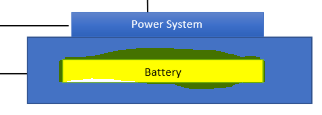
\includegraphics[width=0.60\textwidth]{images/Capture.png}
 \caption{Power layer subsystem diagram}
\end{figure}




\newpage
\section{Frame and Component Layer Subsystems}
In this section, the layer is described in some detail in terms of its specific subsystems. Describe each of the layers and its subsystems in a separate chapter/major subsection of this document. The content of each subsystem description should be similar. Include in this section any special considerations and/or trade-offs considered for the approach you have chosen.

\subsection{Subsystem 1}
This section should be a general description of a particular subsystem for the given layer. For most subsystems, an extract of the architectural block diagram with data flows is useful. This should consist of the subsystem being described and those subsystems with which it communicates.

\begin{figure}[h!]
	\centering
 	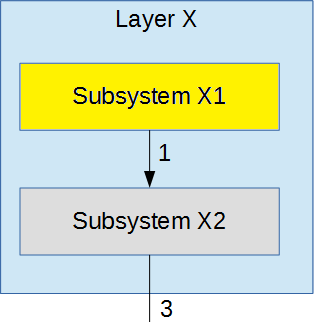
\includegraphics[width=0.60\textwidth]{images/subsystem}
 \caption{Example subsystem description diagram}
\end{figure}

\subsubsection{Assumptions}
Any assumptions made in the definition of the subsystem should be listed and described. Pay particular attention to assumptions concerning interfaces and interactions with other layers.

\subsubsection{Responsibilities}
Each of the responsibilities/features/functions/services of the subsystem as identified in the architectural summary must be expanded to more detailed responsibilities. These responsibilities form the basis for the identification of the finer-grained responsibilities of the layer's internal subsystems. Clearly describe what each subsystem does.

\subsubsection{Subsystem Interfaces}
Each of the inputs and outputs for the subsystem are defined here. Create a table with an entry for each labelled interface that connects to this subsystem. For each entry, describe any incoming and outgoing data elements will pass through this interface.

\begin {table}[H]
\caption {Subsystem interfaces} 
\begin{center}
    \begin{tabular}{ | p{1cm} | p{6cm} | p{3cm} | p{3cm} |}
    \hline
    ID & Description & Inputs & Outputs \\ \hline
    \#xx & Description of the interface/bus & \pbox{3cm}{input 1 \\ input 2} & \pbox{3cm}{output 1}  \\ \hline
    \#xx & Description of the interface/bus & \pbox{3cm}{N/A} & \pbox{3cm}{output 1}  \\ \hline
    \end{tabular}
\end{center}
\end{table}

\subsection{Subsystem 2}
Repeat for each subsystem

\subsection{Subsystem 3}
Repeat for each subsystem


\newpage
\section{MIDI Layer Subsystems}
In this section, the layer is described in some detail in terms of its specific subsystems. Describe each of the layers and its subsystems in a separate chapter/major subsection of this document. The content of each subsystem description should be similar. Include in this section any special considerations and/or trade-offs considered for the approach you have chosen.

\subsection{Subsystem 1}
This section should be a general description of a particular subsystem for the given layer. For most subsystems, an extract of the architectural block diagram with data flows is useful. This should consist of the subsystem being described and those subsystems with which it communicates.

\begin{figure}[h!]
	\centering
 	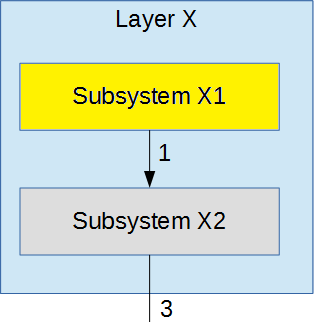
\includegraphics[width=0.60\textwidth]{images/subsystem}
 \caption{Example subsystem description diagram}
\end{figure}

\subsubsection{Assumptions}
Any assumptions made in the definition of the subsystem should be listed and described. Pay particular attention to assumptions concerning interfaces and interactions with other layers.

\subsubsection{Responsibilities}
Each of the responsibilities/features/functions/services of the subsystem as identified in the architectural summary must be expanded to more detailed responsibilities. These responsibilities form the basis for the identification of the finer-grained responsibilities of the layer's internal subsystems. Clearly describe what each subsystem does.

\subsubsection{Subsystem Interfaces}
Each of the inputs and outputs for the subsystem are defined here. Create a table with an entry for each labelled interface that connects to this subsystem. For each entry, describe any incoming and outgoing data elements will pass through this interface.

\begin {table}[H]
\caption {Subsystem interfaces} 
\begin{center}
    \begin{tabular}{ | p{1cm} | p{6cm} | p{3cm} | p{3cm} |}
    \hline
    ID & Description & Inputs & Outputs \\ \hline
    \#xx & Description of the interface/bus & \pbox{3cm}{input 1 \\ input 2} & \pbox{3cm}{output 1}  \\ \hline
    \#xx & Description of the interface/bus & \pbox{3cm}{N/A} & \pbox{3cm}{output 1}  \\ \hline
    \end{tabular}
\end{center}
\end{table}

\subsection{Subsystem 2}
Repeat for each subsystem

\subsection{Subsystem 3}
Repeat for each subsystem


\newpage
\section{Sound Modules Layer Subsystems}
This layer is responsible for reading the MIDI signals and converting it into audio signals that is needed for the speakers to produce audio output. It consists of MIDI decoder, fluid synth and sound card which are integrated in a Raspberry Pi.

\subsection{Layer Hardware}
It consists of 1.5GHZ quad-core 64-bit raspberry pi.

\subsection{Layer Operating System}
It runs raspbian OS with kernel version 4.19.

\subsection{MIDI Decoder}
It is a driver program that acts as an bridge program between MIDI encoder and the fluidsynth.

\begin{figure}[h!]
	\centering
 	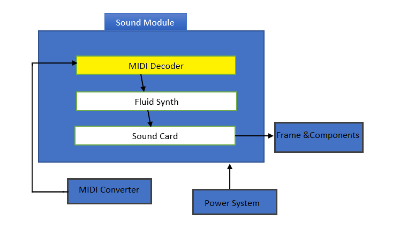
\includegraphics[width=0.60\textwidth]{images/decoder.png}
 \caption{MIDI decoder subsystem description diagram}
\end{figure}

\subsubsection{Subsystem Hardware}
It is running on Raspberry pi 4.

\subsubsection{Subsystem Operating System}
Raspbian OS is running a python 3.6 script that reads the encoding.

\subsubsection{Subsystem Programming Languages}
It uses Python 3.6.0 for server processing which uses socket library for communication with fluidsynth. 

\subsection{Fluidsynth}
Fluidsynth is a real-time MIDI synthesizer based on the SoundFont 2 specifications. 

\begin{figure}[h!]
	\centering
 	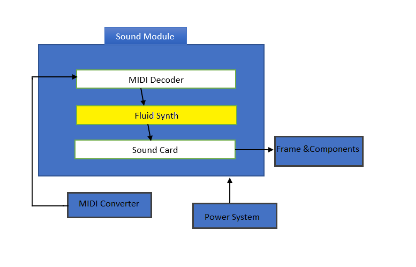
\includegraphics[width=0.60\textwidth]{images/fluidsynth.png}
 \caption{Fluidsynth subsystem description diagram}
\end{figure}

\subsubsection{Subsystem Operating System}
It is runs on startup on a raspbian OS.

\subsubsection{Subsystem Software Dependencies}
Fluidsynth is a library itself which reads in the MIDI input and plays according to the sound font files present. Moreover, socket library is called upon to connect with the fluidsynth process which in turn uses AF\_INET IPV4 protocol for communication.

\subsubsection{Subsystem Programming Languages}
Python is used to call upon the fluidsynth functions to control the gain, reverb and chorus of the audio output. M

\subsection{Soundcard}
Raspberry pi already comes in with a sound card integrated in its system. It is used for converting the output data from fluidsynth to audio data used by speakers for final output.

\begin{figure}[h!]
	\centering
 	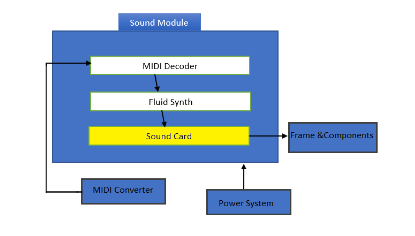
\includegraphics[width=0.60\textwidth]{images/sound card.png}
 \caption{Sound Card subsystem description diagram}
\end{figure}

\subsubsection{Subsystem Hardware}
Raspberry pi 4 with compatible sound drivers for necessary sound processing.

\subsubsection{Subsystem Operating System}
Raspbian OS 









\newpage
\newpage
\section{User Interface}
This layer allows the user to control the sound font files to use such as church,acoustic guitar,etc. Also, it allows the user to change the reverb, gain and chorus of the sound as well as switch back and forth between the presets.

\subsection{Layer Hardware}
Elecrow 5 inch capacitive touch screen with 800*480 TFT LCD display is used as an interactive medium with the user.

\subsection{Layer Operating System}
It depends on the Raspbian OS.

\subsection{Layer Software Dependencies}
Python 3.6 is used to create the GUI for the application which uses tkinter library to create the button and sliders to control the audio output.  




\newpage

\section{Appendix A}
Include any additional documents (CAD design, circuit schematics, etc) as an appendix as necessary.
\newpage


%%% References
\bibliographystyle{plain}
\bibliographystyle{reference/IEEEtran_custom}
\bibliography{reference/refs}{}
  Fluidsynth manpage-https://manpages.debian.org/testing/fluidsynth/fluidsynth.1.en.html 

\\*Tkinter- http://effbot.org/tkinterbook/


\end{document}